\chapter{虚拟网络嵌入问题}
\section{SDN网络虚拟化概述}
现如今未来互联网架构提案存在两种主要方法:一元论和多元论。首先,一元论模型 中网络有一个整体架构,架构必须足够灵活,以支持所有将会出现的网络应用。在一元论网络架构方法中,每次当且仅当一个协议栈运行在物理层上。而多元论的思想是基于互联网必须同时支持多个网络,每个网络具有运行协议栈的能力,该协议栈是适合一项给定应用需求的。这种针对特定服务而创建特定网络的做法,简化了例如移动性、安全性或服务质量等特性的新应用的部署,为提供不同服务而设计多个网络的做法比为同时处理不同服务而设计一个独特网络的做法要更简单高效。 因此,多元论方法可以被理解为是一种“分而治之”方法的。因为寻找涵盖所有可能需求的单一解决方案是非常困难的,构造支持这些需求的网络就成为了一种可行的替代方法,这是多元论架构的首要特点,多元论被广泛接受的原因是一元论方法不仅能解决所有己知的互联网问题,而且也能要求在未来网络的演进过程中依然能够持续运行。此外,多元论的另一个关键优势就是其固有的后向兼容性,因为当前的互联网是可以并行运行的。多元论提案是基于多个网络运行在同一基础设施之上的同一思想,即使它们在寻址方案、报文格式和协议方面存在差异,也是如此,因为这些网络共享一个物理层,例如链路和路由器等,所以对基础介质的多种访问方式必须由同一个检测器进行编排。这个检测器就是一个特殊应用的软件,它将共享介质虚拟化后提供给运行在其上的多个网络,因此每个网络的运行就像它正在使用给定的物理资源一样,这些网络就是虚拟网络,但是为了能够共享一个物理底层,这将不得不面临网络性能的挑战。

虚拟化是以软件模拟硬件平台如服务器、网络资源或存储设备等功能,所有功能都与硬件解耦分离,并被模拟为“虚拟实例”,具有像传统的硬件解决方案一样的操作能力。此外可以使用单个硬件平台来支持多个虚拟机器或设备,这些虚拟机器或设备根据需求容易改变,因此与传统的基于硬件的解决方案相比,虚拟化解决方案的可扩展性,可移植性和成本效益更高。

计算机虚拟化主要是应用在数据中心,可以在一台物理机上同时运行几台服务器。计算机虚拟化与网络虚拟化比较类似,支持网络虚拟化共享的资源是网络。将虚拟化技术应用到网络的最主要动机是尽量在每个虚拟网络也即虚拟分片内运行各自定制的协议栈。 在计算机中,网络虚拟化是将软件和硬件的网络功能和网络资源组合成基于软件的单个管理实体。

网络虚拟化包括平台虚拟化,通常与资源虚拟化相结合。另外,网络虚拟化通常分为内部虚拟化和外部虚拟化。内部虚拟化是为单个网络服务器上的软件容器提供类似网络的功能,使用伪接口或软件容器配置单个系统,以使用软件仿真物理网络,这可以通过将应用程序隔离到伪接口或单独容器来提高单个系统的效果。外部虚拟化将网络或网络的部分组合成虚拟单元,将一个或多个局域网(LAN)组合为虚拟网络,可以提高数据中心或大型网络的效率,虚拟局域网(VLAN)和网络交换机包括关键组件。使用此技术,系统管理员可以将在物理上连接到同一本地网络的系统配置为单独虚拟网络。相反,管理员可以将单独的局域网(LAN) 上的系统组合成跨越大网络段的单个VLAN。



数据中心网络需要虚拟化,就像计算和存储的虚拟功能一样,这样可以很高效方便地隔离共存的多个租户。现有的数据中心网络虚拟化经历了两个阶段:第一阶段是使用简单的VLAN和MAC 地址来实现隔离:第二阶段的是使用IP覆盖网络,这两个阶段的方法都有各自对应的缺陷,首先,基于VLAN 和MAC 地址的方法难以配置和管理,并且将虚拟机网络与物理基础设施直接绑定会使得虚拟机的放置和挪动不够灵活。其次,IP覆盖网络对参与虚拟网络的虚拟机数量有限制,并且出现的故障问题难以调试。现在行业提出了一种新的方法,利用多层标签来实现隔离网络,并且可以指定通过数据屮心网络的路由,分组标签可以使用SDN控制平面,控制平面实现了数据中心交换机的OpenFlow控制。


当虚拟化应用于网络时,虚拟化可以创建硬件和软件网络资源(路由器、交换机等)的基于软件化的逻辑视图。物理网络设备简单地负责分组的转发,而虚拟网络提供智能抽象,这样有利于部署以及管理网络服务和底层网络资源。因此,网络虚拟化可以调整网络以更好地支持虚拟化环境。


在网络虚拟化环境中,多个异构的虚拟网络架构都共享底层物理网设施,这种共享是对底层物理网络设施进行隔离、抽象而形成的。不同的虚拟网络在很多方面都是不同的:服务的提供、网络拓扑、技术的使用等。网络虚拟化主要是想要 极大地发挥资源共享的优势,支持未来网络发展的渐进部署,进行灵活的配置与管理。相比于现有的互联网,这种体系架构优劣分明:它提供了确保了安全性和服务质量,更灵活的资源供使用;但与此同时,我们也需要设计一套更加 完善和复杂的虚拟网络管理机制来保证 这种性能改善。

在虚拟网络中有三个角色:基础设施提供商、服务提供商和客户。每个角色 都有不同的目标:基础设施提供商通常专注于平衡负载,最大化收入和最小化成 本;服务提供商通常关注最大化收入,例如,尽可能多地支持客户或请求,他们 是客户和基础设施提供商之间的中介;客户通常专注于服务质量,例如下载时间 或比特率。也就是说,网络虚拟化的一个优点是虚拟网络可具有异构资源以满足 各种定制需求,虚拟化也可以提供实验环境为研宄人员评估新的协议。当服务提 供商生成虚拟网络请求时,它可以为每个虚拟节点和链路指定资源。因此,当将 虚拟网络请求嵌入到底层网络中特定的物理节点和链路上时,其必须满足对虚拟 节点和虚拟链路的约束。

%未来的互联网架构将基于基础设施即服务(IaaS)\cite{bhardwaj2010cloud}业务模型,将当前互联网服务提供商(ISP)的角色解耦为两个新角色:部署和维护网络设备的基础设施提供商(InP)和服务提供商(SP)负责部署网络协议并提供端到端服务。网络虚拟化的引入分离三个主要参与者(参见图\ref{fig:FutureInternetBusinessModel})为SP\cite{schaffrath2009network} 的管理和业务角色:虚拟网络提供者(VNP),该虚拟网络提供者(VNO)从一个或多个IPS组装虚拟资源,安装、管理虚拟网络运营商(VNO)。并根据SP 的需要,运行VN,使用VNS 进行业务管理,集中管理业务。

%\begin{figure}[htbp]
%\centering
%% Requires \usepackage{graphicx}
%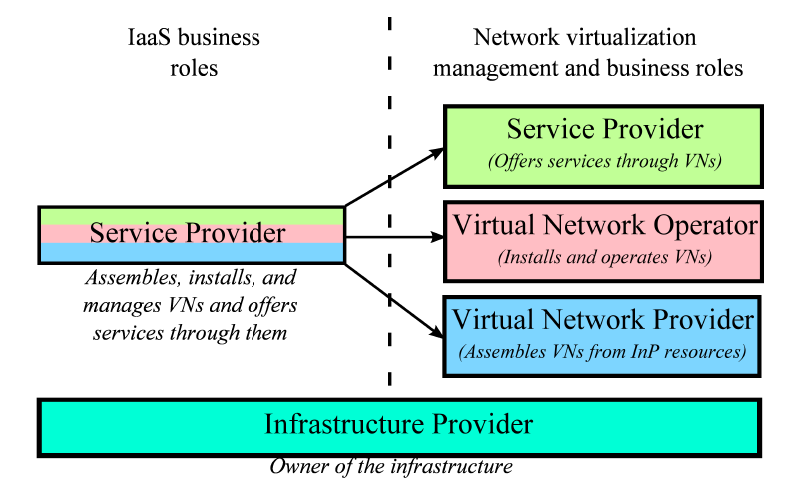
\includegraphics[width=3.0in]{figures/FutureInternetBusinessModel}
%  \caption{未来互联网商业模式}
%  \label{fig:FutureInternetBusinessModel}
%\end{figure}




\section{网络虚拟化的技术特征}
网络虚拟化也是现在网络领域的一研究方向,总的来说,它具有如下特征:
\begin{enumerate}
  \item 独立性:网络虚拟化平台的运行不受网络硬件的限制,而且未来出现的 网络架构会更好地支持虚拟化和商品化,从而能够进一步改善云的成本代价。
  \item 隔离性:底层物理网络、控制平面和虚拟网络之间要进行安全隔离,通过共享底层物理资源,能够大大地提高计算能力,并且可以优化存储资源和网络资源的使用率。网络虚拟化平台在进行资源整合的同时还必须提供隔离,同时也要隔离虚拟网络的地址和底层物理网络。
  \item 多功能性:可以很好地复制物理网络的服务模式,对于运行在任一物理环境下的任一工作负载,网络虚拟化平台必须能够提供很好的支持,此外,对于现有的网络 服务,比如负载均衡,WAN优化以及ACL 等,也必须要能够提供。
  \item  灵活性:网络虚拟化要遒循计算领域虚拟化的模式,在计算领域,虚拟机能够被 作为一个软状态来进行处理,这是该领域虚拟化的一个主要特征,网络虚拟化也 必须要具有同样的灵活性。
  \item   可测试性:网络虚拟化要具有云的规模和性能,网络虚拟化要有能力支持大规模的 网络部署环境,这样不仅可以允许存在大量的租户,而且还可以支持很多服务, 如数据中心的租用等。网络虚拟化还不应该允许网络中存在故障点或拥寒点,并 且可以支持故障切换功能和多路由功能。
  \item 兼容性,网络虚拟化平台要能够与任何的hypervisor平台兼容。
\end{enumerate}


\section{虚拟网络嵌入算法}
在网络虚拟化中,主要实体是虚拟网络(VirtualNetwork,VN)。VN是顶部的主动式和被动式网络元素(网络节点和网络链路)的组合。物理网络(SN)。虚拟节点通过虚拟链路互连,形成虚拟拓扑。通过虚拟化SN的节点和链接资源,多个虚拟可以在相同的物理硬件上创建和共同管理具有广泛变化特性的网络拓扑。此外,资源虚拟化机制引入的抽象允许网络运营商以高度灵活和动态的方式管理和修改网络。

网络虚拟化技术通过对物理网络资源进行抽象、隔离和分配,可支持多个虚 拟网络共存于同一物理网络中。在底层网络中嵌入虚拟网络是网络虚拟化面临的主要是资源分配问题,通常被称为虚拟网络嵌入(Virtual Network Embedding,VNE)问题。通过动态嵌入将虚拟资源转移到物理硬件上,可以最大限度地利用现有硬件的好处。虚拟网络嵌入是实现网络虚拟化的关键,旨在研究如何合理地将租户定制的虚拟网络请求嵌入嵌入到底层物理网络中,获取满足虚拟 网络服务所需要的物理网络资源,从而提高网络资源利用率和虚拟网络请求接受率。。最优的动态资源分配,导致未来网络的自配置和组织。为终端用户提供定制的端到端保证服务.这种最优性可以根据不同的目标来计算,从QoS、经济效益、生存性到网络的安全性。图\ref{fig:ResourceAllocationInFutureInternet}说明网络虚拟化如何使用嵌入算法,以便以最佳方式在物理基础设施上分配虚拟资源。VNO使用嵌入算法来决定从哪个虚拟资源请求。VNP 通过使用InPS衬底资源来实例化它们。
\begin{figure}[htbp]
\centering
% Requires \usepackage{graphicx}
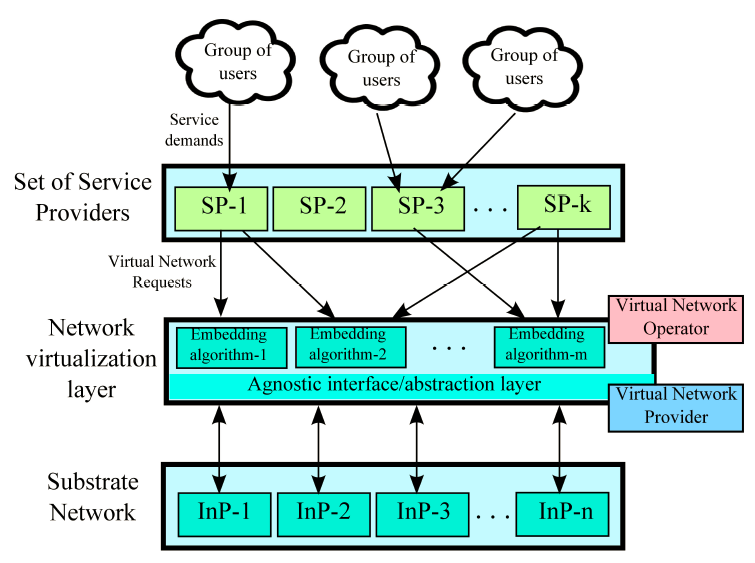
\includegraphics[width=3.0in]{figures/ResourceAllocationInFutureInternet}
  \caption{未来互联网的资源配置}
  \label{fig:ResourceAllocationInFutureInternet}
\end{figure}

虚拟网络嵌入涉及节点和链路中虚拟资源的分配。因此,它可以分为两个子问题:虚拟节点嵌入(VNoM),其中虚拟节点必须在物理节点中分配。虚拟链路嵌入(VLiM),其中连接这些虚拟节点的虚拟链路必须嵌入到底层网络中相应节点的路径。虚拟网络的一个 节点能够被嵌入到物理网络拓扑中的任意一个物理节点,并且一条虚拟链路也可能会被嵌入到底层物理网的多条物理路径,因此,任意一个虚拟网络被嵌入到底 层物理网络时,都会有多种嵌入方案。所以怎么把业务供应商的虚拟网络请求与物理网络进行嵌入就显得尤为重要。当虚拟网络的链路和节点有约束条件时,此时的嵌入算法属于NP难问题\cite{amaldi2016computational},即使是考虑最简单的没有约束条件的情况,在虚拟 网络拓扑给定的情况下,也仍然是NP难问题\cite{amaldi2016computational}。所以现在在大多的研宂中,基本是 利用启发式算法来求解虚拟网络的嵌入问题,尽量优化解决方案。



简单算法嵌入是虚拟网络嵌入相关问题的基础,没有考虑底层设备的故障和 复杂的基础设施构成,也没有考虑虚拟网络请求的在线达到。在将虚拟链路嵌入到底层物理路径上时,如果允许路径分割,那么一条虚拟链路将会嵌入到底层物 理网络的多条路径上,这些路径的源目的节点相同,并且在链路嵌入时,物理链 路需要有足够的带宽\cite{yu2008rethinking}。在一次虚拟网络请求嵌入在物理网之后,物理网的剩余 节点的计算资源和链路的带宽容量将会相应地减少。在虚拟网络的请求是已知的情况下,此时的虚拟网络嵌入问题可以转化为多路分离器(multiway separator)问题求解,是一个NP难问题\cite{andersen2002theoretical}。

VNE问题有多种不同变体。因此,文献中提出的所有VNE方法都可以根据它们是静态的还是动态的、集中的还是分布的、简洁的还是冗余的进行分类。这六个概念将在这里描述。
\begin{enumerate}
  \item 静态vs动态:在大多数现实世界中,VNE必须作为网络问题来解决.也就是说,不会事先知道虚拟网络请求(VNR)的到来。相反,虚拟网络动态地到达系统,并且可以在网络中停留任意时间。为了实际起见,VNE算法必须在VNR到达时处理它们,而不是一次加入一组VNR(脱机VNE)。 虽然原则上所有方法都可以在线操作,但静态VNE 方法并不考虑重新映射更多VNR之一的可能性,以提高SN中嵌入的性能。一些影响导致需要重新安置部分(甚至是完整的)虚拟网络:比如底层网络资源的破碎化,虚拟网络的变化,底层网络的更改。

      动态VNE方法试图重新配置映射的虚拟网络请求,以便重新组织资源分配并优化底层网络资源的使用。例如,图\ref{fig:RelocationMappedVNRsOnlineVNE}显示了在不同时间到达并离开底层网络的三个VNR 的在线嵌入。如果底层网络资源不是第一次通过重新配置已映射的VNR2来去碎片,则它们中的最后一个VNR3不能嵌入。


  \item 集中式vs分布式:VNE问题可以通过集中式或分布式方式解决。每一种方法都有其各自的优点和缺点,从根本上说是不同的。
  \item 简洁vs冗余:单个底层网络实体的失败将影响映射到它的所有虚拟实体。因此,在故障敏感的应用程序部署在虚拟网络内的环境中,可以设置备份资源,在相应的主要资源失败的情况下,这些资源可以用作回退资源。要做到这一点,嵌入结果本身可以是冗余的,对于节点和/或链路故障是有弹性的。否则,如果没有冗余嵌入结果被称为“简洁”。
\end{enumerate}

\begin{figure}[htbp]
\centering
% Requires \usepackage{graphicx}
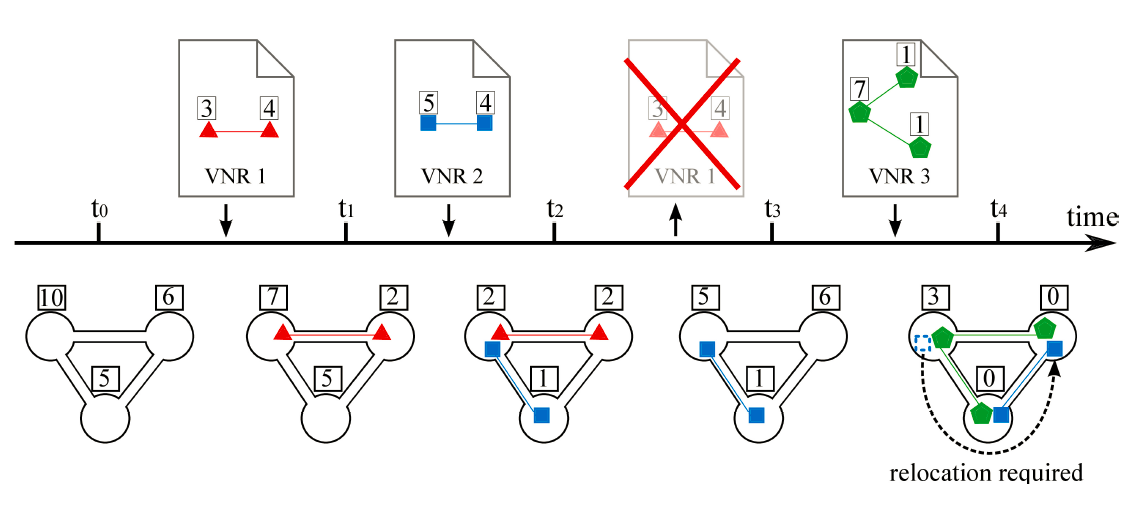
\includegraphics[width=3.0in]{figures/RelocationMappedVNRsOnlineVNE}
  \caption{在线VNE算法中重新映射VNR}
  \label{fig:RelocationMappedVNRsOnlineVNE}
\end{figure}

每个类别都是相互独立的。例如,一个算法可以同时具有集中式、动态性和冗余性。在此基础上,可以导出一个泛型表示法来确定用以下语法描述:

\begin{center}
  $[C|D]/[S|D]/[C|R]$
\end{center}

第一个字符表示算法是集中的还是分布式的。同样,第二个字符表示算法是静态的还是动态的。最后,第三个字符表示该算法是简洁的还是冗余的。因此,表示为C/D/R的算法将是一种集中式的、动态的、冗余的算法。这样就可以对任何给定的算法进行快速分类,并与类似的方法进行适当的比较。

总之,表\ref{tab:TaxonomyOfConciseVNEApproach}给出了虚拟网络嵌入算法简明的分类。
\wuhao\begin{longtable}{lllll}
\caption{虚拟网络嵌入算法分类}\label{tab:TaxonomyOfConciseVNEApproach}
 \vspace{0.5em}\\
\toprule[1.5pt]
类型   & 论文  & 优化 & 协调 & 贡献  \\
\midrule[1pt]
\endfirsthead
\multicolumn{5}{c}{表~\thetable(续表)}\vspace{0.5em}\\
\toprule[1.5pt]
类型   & 论文  & 优化 & 协调 & 贡献  \\
\midrule[1pt]
\endhead
\bottomrule[1.5pt]
\endfoot
\multirow{28}{*}{C/S/C} & Inführ and Raidl (2011)\cite{infuhr2011introducing}  & Exact & One Stage & 提供延迟、位置和路由约束。 \\
 & Liu et al. (2011)\cite{liu2011completing}  & Exact & One Stage & 基于对应矩阵的精确VNE\\
 & Trinh et al. (2011)\cite{trinh2011quality}  & Exact & One Stage & 具有SLA QoS保证的精确VNE问题\\
 & Pages et al. (2012)\cite{pages2012strategies}  & Exact/Metaheuristic & One Stage & 介绍了光网络中的VNE\\
 & Lischka and Karl (2009)\cite{lischka2009virtual}  & Heuristic & One Stage & 提供基于SID一个阶段的VNE\\
 & Di et al. (2010)\cite{di2010cost}  & Heuristic & One Stage & 改进\cite{lischka2009virtual} 方法\\
 & Ghazar and Saaman (2011)\cite{ghazar2011hierarchical}  & Heuristic & One Stage & 介绍SN的分层管理\\
 & Yun et al. (2011-2012)\cite{yun2011virtual,yun2013embedding}  &Heuristic & One Stage & 第一种在无线多跳网络中的VNE方法,介绍无线VNE的度量和可行性措施\\
 & Chen et al. (2012)\cite{chen2012virtual}  & Heuristic & One Stage & 减少资源碎片\\
 & Yu et al. (2012)\cite{yu2012cost}  & Heuristic & One Stage & 增加协调的一步VNE\\
 & Liu et al. (2011)  & Heuristic & Two Stages & 基于节点邻近的改进协调\\
 & Sheng et al. (2011-2012)  & Heuristic & a & a\\
 & Li et al. (2012)  & Heuristic & a & a\\
 & Lu and Turner (2006)  & Heuristic & a & a\\
 & Yu et al.* (2008)  & Heuristic & a & a\\
 & Razzaq and Siraj (2010)  & Heuristic & a & a\\
 & Razzaq et al. (2011)  & Heuristic & a & a\\
 & Nogueira et al. (2011)  & Heuristic & a & a\\
 & Leivadeas et al.* (2011)  & Heuristic & a & a\\
 & Botero et al. (2011-2013)  & Heuristic & a & a\\
 & Zhu and Ammar* (2006)  & Heuristic & a & a\\
 & Fajjari et al. (2011)  & Metaheuristic & a & a\\
 & Cheng et al. (2012)  & Metaheuristic & a & a\\
 & Zhang et al. (2012)  & Heuristic & a & a\\
 & Di et al. (2012)  & Heuristic & a & a\\
 & Abedifar and Eshghi (2012)  & Heuristic & a & a\\
 & Aris Leivadeas et al. (2012)  & Heuristic & a & a\\
 & Tae-Ho Lee et al. (2012)  & Heuristic & a & a\\
\hline
\multirow{7}{*}{C/D/C} & Fajjari et al. (2011)  & Heuristic & a& a\\
 & Bienkowski et al. (2010)  & Heuristic & a & a\\
 & Zhu and Ammar* (2006)  & Heuristic & a & a\\
 & Fan and Ammar (2006)  & Heuristic & a & a\\
 & Cai et al. (2010)  & Heuristic & a & a\\
 & Shun-li and Xue-song (2011)  & Heuristic & a & a\\
 & Sun et al. (2012)  & Heuristic & a & a\\
\hline
\multirow{5}{*}{D/S/C} & Houidi et al. (2010)  & Heuristic & a& a\\
 & Xin et al. (2011)  & Heuristic & a & a\\
 & Lv et al. (2011)  & Heuristic & a & a\\
 & Houidi et al.* (2011)  & Exact/Metaheuristic & a & a\\
 & Leivadeas et al.* (2012)  & Heuristic & a & a\\
\hline
\multirow{1}{*}{D/D/C} & Marquezan et al. (2010)  & Heuristic  & a& a\\
\hline
\multirow{31}{*}{C/S/R} & Houidi et al.* (2011)  & Exact & a& a\\
 & Zhang et al. (2011)  & Exact & a & a\\
 & Botero et al. (2012)  & Exact & a & a\\
 & Wang and Wolf (2011)  & Exact & a & a\\
 & Shamsi and Brockmeyer(2007-2009)  & Heuristic & a & a\\
 & Koslovski et al. (2010)  & Heuristic & a & a\\
 & Yu et al. (2010)  & Heuristic & a & a\\
 & Lv et al. (2012)  & Heuristic & a & a\\
 & Chowdhury et al. (2009-2011)  & Heuristic & a & a\\
 & Rahman et al. (2010)  & Heuristic & a & a\\
 & Butt et al.* (2010)  & Heuristic & a & a\\
 & Yeow et al. (2010)  & Heuristic & a & a\\
 & Sun et al. (2011)  & Heuristic & a & a\\
 & Yu et al. (2011)  & Heuristic & a & a\\
 & Yu et al.* (2008)  & Heuristic & a & a\\
 & Gao et al. (2010)  & Heuristic & a & a\\
 & Yang et al. (2010)  & Heuristic & a & a\\
 & Zho et al. (2010)  & Heuristic & a & a\\
 & Chen et al. (2010)  & Heuristic & a & a\\
 & Yu et al. (2011)  & Heuristic & a & a\\
 & Sun et al. (2011)  & Heuristic & a & a\\
 & Lu et al. (2011)  & Heuristic & a & a\\
 & Guo et al. (2011)  & Heuristic & a & a\\
 & Cheng et al. (2011)  & Metaheuristic & a & a\\
 & Sheng et al. (2011)  & Metaheuristic & a & a\\
 & Zhang et al. (2012)  & Metaheuristic & a & a\\
 & Sun et al. (2012)  & Metaheuristic & a & a\\
 & Lv et al. (2012)  & Metaheuristic & a & a\\
 & Leivadeas et al.* (2012)  & Heuristic & a & a\\
 & Masti and Raghavan (2012)  & Heuristic & a & a\\
 & Zhang et al. (2012)  & Exact/Heuristic & a & a\\
\hline
\multirow{4}{*}{C/D/R} & Butt et al.* (2010)  & Heuristic & Two Stages & a\\
 & Yu et al.* (2010)  & Heuristic & Uncoordinated & a\\
 & Schaffrath et al. (2010)  & Exact& One Stage & a\\
 & Chen et al. (2011)  & Heuristic & Two Stages & a\\
\hline
\multirow{1}{*}{D/S/R} & Chowdhury et al. (2010)  & Heuristic & InterInP & 第一次提出INP-VNE算法。在InP 和SP收益之间进行协调。VNR在不同InPs中划分和在各自的本地InPS嵌入\\
\hline
\multirow{1}{*}{D/D/D} & Houidi et al. (2010)  & Heuristic & Two Stages& 针对节点和链路故障的容错VNE\\
\end{longtable}\xiaosi
\vspace{\baselineskip}


\section{可生存虚拟网络嵌入算法}
根据是否对租户的虚拟网络提供备份资源,可以将SVNE算法划分为两类: 基于主动保护策略的算法和基于被动恢复策略的算法\cite{herker2013survey}。

在基于主动保护策略的算法中,在嵌入虚拟网络请求前,为虚拟网络预置备份资源,以供后续故障恢复使用。该策略可以提供较高的虚拟网络生存性保障, 但是对于备份资源消耗较大。代表性算法如:FI-EVN\cite{yu2011cost}、FD-EVN\cite{wang2014survivable} LC-SVNE\cite{hu2012location} 等。

在基于被动恢复策略的算法中,在嵌入虚拟网络请求前,不预置备份资源, 在后续故障发生后再使用节点迁移或者现有的物理网络资源进行故障恢复。该策 略的优势在于不需要额外提供虚拟网络备份资源,但是相对而言,故障恢复成功 率不稳定且恢复效率较低。代表性算法如:NB-SVNE\cite{bo2014dynamic}、MR-SVNE\cite{qiang2014heuristic} 等。

SVNE算法的两种备份策略均存在性能问题,其中主动保护策略需要提供虚拟网 络全部重要节点及其关联链路的备份资源,所以该策略的虚拟网络请求接受率较 低,被动恢复策略每次进行故障发生时需要使用现有网络资源进行故障恢复,故障恢复效率低下。

总之,表\ref{tab:survivableVirtualNetworkEmbedd}给出了可生存虚拟网络嵌入算法的比较。
\begin{table}[htbp]
\caption{可生存虚拟网络嵌入算法总结}\label{tab:survivableVirtualNetworkEmbedd}
\vspace{0.5em}\centering\wuhao
\begin{tabularx}{48em}{|*{4}{>{\centering\arraybackslash}X|}}
\toprule[1.5pt]
算法(论文)   & 故障类型  & 优化目标 & 处理机制  \\
\midrule[1pt]
Survivable virtual network embedding\cite{rahman2013svne} & 单个物理链路失效 & 为基础设施提供最大限度的收入 & 被动,失效后(Restoration)\\
\hline
Shared backup network provision for virtual network embedding\cite{guo2011shared} & 单个物理链路失效 & 最大化收益/VN接受率& 主动,失效前(Protection)\\
\hline
Migration based protection for virtual infrastructure survivability for link failure\cite{yu2011migration} & 单个物理链路失效 & 最小化成本 & Protection\\
\hline
QoSMap: Achieving Quality and Resilience through Overlay Construction\cite{shamsi2009qosmap} & 单个物理链路失效 & 尽量减少额外备份资源和延迟 & Protection\\
\hline
An overlay mapping model for achieving enhanced QoS and resilience performance\cite{zhang2011overlay};An overlay mapping model for achieving enhanced QoS and resilience performance\cite{zhang2011overlay} & 单个物理链路失效 & 尽量减少额外备份资源和延迟 & Protection\\
\hline
Cost efficient design of survivable virtual infrastructure to recover from facility node failures\cite{yu2011cost} & 单个虚拟节点故障& 最小化成本 & Protection\\
\hline
A novel two-step approach to surviving facility failures\cite{qiao2011novel} & 单个虚拟节点故障 & 尽量减少资源/总成本 & Protection\\
\hline
Survivable virtual infrastructure mapping in a federated computing and networking system under single regional failures\cite{yu2010survivable} & 单个区域失效 & 最小化成本 & Protection \\
\hline
Location-constrained survivable network virtualization\cite{hu2012location} & 单个虚拟节点故障 & 尽量减少资源 & Protection\\
\hline
Designing and embedding reliable virtual infrastructures\cite{yeow2010designing} & 单个物理节点故障 & 尽量减少所用资源 & Protection\\
\hline
Survivable virtual infrastructure mapping in virtualized data centers\cite{xu2012survivable} & 单个服务器故障 & 最小化运营成本& Protection\\
\hline
Adaptive virtual network provisioning\cite{houidi2010adaptive} & 单个节点或者链路故障 & 最小化通信成本 & Restoration\\
\bottomrule[1.5pt]
\end{tabularx}
\vspace{\baselineskip}
\end{table}

\section{算法评价指标}
生存性虚拟网络嵌入算法的最终目标是实现网络运营收益最大化和成本消 耗最小化。因此,为了实现网络运营收益最大化,需要在提高虚拟网络嵌入收益的同时,保障较高的故障恢复成功率和恢复效率以降低故障成本。

度量标准对于评估成功嵌入的质量是必要的。它们用于比较不同的VNE方法,并量化优化方面的进展。在本调查文件中,不同的度量被分成以下四大类别:

通过对虚拟网络嵌入(VNE)算法文献的调研,选取了算法性能分析常用的八组评价指标作为实验性能参数,分别是:
\begin{itemize}
  \item 服务质量度量
  \item 成本相关度量
  \item 可生存性度量
  \item 其他度量
\end{itemize}
表\ref{tab:MetricsForVirtualNetworkEmbedding}概述了本文讨论的各种指标。根据应用程序场景,可以为大多数度量计算平均值、最大值和/或最小值。
\begin{table}[htbp]
\caption{虚拟网络嵌入的度量}\label{tab:MetricsForVirtualNetworkEmbedding}
\vspace{0.5em}\centering\wuhao
\begin{tabular}{lll}
\toprule[1.5pt]
优化目标  & 度量   & 描述  \\
\midrule[1pt]
\multirow{6}{*}{服务质量} & Path Length  & 平均由虚拟链路跨越的底层链路数\\
 & Stress level  & 底层网络实体实现的虚拟实体的数量\\
 & Utilization & 嵌入的全部物理资源和物理网络链路总数的比值\\
 & Throughput & 虚拟节点之间可实现的数据速率\\
 & Delay  & 一个数据包通过虚拟链路所用的时间
\\
 & Jitter  & 虚拟链路上数据包到达时间的变化\\
\hline
\multirow{4}{*}{资源支出} & Cost  & 嵌入VNRS的所有底层网络资源之和\\
 & Revenue  & VNRs的所有所需资源之和\\
 & Cost/Revenue & 底层网络资源与所提供虚拟网络资源的比率\\
 & Acceptance ratio & 嵌入成功的虚拟网络请求数和全 部虚拟网络请求数目的比值\\
\hline
\multirow{6}{*}{可生存性} & Number of backups  &可用备份资源的数量\\
 & Path redundancy  & 多路径嵌入中路径的多样性\\
 & Cost of resilience & 维护可生存性所需的额外节点数\\
 & Recovery blocking probability & 不可恢复的故障场景与所有故障情景的比率\\
 & Number of migrations  & 在发生故障时必须移动的虚拟节点数\\
 & Failure Recovery ratio  & 恢复成功的全部虚拟和发生 障的全部虚拟的节点数目比值\\
\hline
\multirow{3}{*}{其它} & Runtime of the algorithm  & VNE算法在嵌入一定大小的数据时所需的时间\\
 & Number of coordination messages  & 为了完成嵌入而必须在分布式环境中交换的消息数量\\
 & Active substrate nodes & 为了实现管理虚拟基础设施,必须打开的底层节点数\\
\bottomrule[1.5pt]
\end{tabular}
\vspace{\baselineskip}
\end{table}

